% Options for packages loaded elsewhere
\PassOptionsToPackage{unicode}{hyperref}
\PassOptionsToPackage{hyphens}{url}
\documentclass[
  11pt,
]{article}
\usepackage{xcolor}
\usepackage[margin=1in]{geometry}
\usepackage{amsmath,amssymb}
\setcounter{secnumdepth}{5}
\usepackage{iftex}
\ifPDFTeX
  \usepackage[T1]{fontenc}
  \usepackage[utf8]{inputenc}
  \usepackage{textcomp} % provide euro and other symbols
\else % if luatex or xetex
  \usepackage{unicode-math} % this also loads fontspec
  \defaultfontfeatures{Scale=MatchLowercase}
  \defaultfontfeatures[\rmfamily]{Ligatures=TeX,Scale=1}
\fi
\usepackage{lmodern}
\ifPDFTeX\else
  % xetex/luatex font selection
\fi
% Use upquote if available, for straight quotes in verbatim environments
\IfFileExists{upquote.sty}{\usepackage{upquote}}{}
\IfFileExists{microtype.sty}{% use microtype if available
  \usepackage[]{microtype}
  \UseMicrotypeSet[protrusion]{basicmath} % disable protrusion for tt fonts
}{}
\makeatletter
\@ifundefined{KOMAClassName}{% if non-KOMA class
  \IfFileExists{parskip.sty}{%
    \usepackage{parskip}
  }{% else
    \setlength{\parindent}{0pt}
    \setlength{\parskip}{6pt plus 2pt minus 1pt}}
}{% if KOMA class
  \KOMAoptions{parskip=half}}
\makeatother
\usepackage{color}
\usepackage{fancyvrb}
\newcommand{\VerbBar}{|}
\newcommand{\VERB}{\Verb[commandchars=\\\{\}]}
\DefineVerbatimEnvironment{Highlighting}{Verbatim}{commandchars=\\\{\}}
% Add ',fontsize=\small' for more characters per line
\usepackage{framed}
\definecolor{shadecolor}{RGB}{248,248,248}
\newenvironment{Shaded}{\begin{snugshade}}{\end{snugshade}}
\newcommand{\AlertTok}[1]{\textcolor[rgb]{0.94,0.16,0.16}{#1}}
\newcommand{\AnnotationTok}[1]{\textcolor[rgb]{0.56,0.35,0.01}{\textbf{\textit{#1}}}}
\newcommand{\AttributeTok}[1]{\textcolor[rgb]{0.13,0.29,0.53}{#1}}
\newcommand{\BaseNTok}[1]{\textcolor[rgb]{0.00,0.00,0.81}{#1}}
\newcommand{\BuiltInTok}[1]{#1}
\newcommand{\CharTok}[1]{\textcolor[rgb]{0.31,0.60,0.02}{#1}}
\newcommand{\CommentTok}[1]{\textcolor[rgb]{0.56,0.35,0.01}{\textit{#1}}}
\newcommand{\CommentVarTok}[1]{\textcolor[rgb]{0.56,0.35,0.01}{\textbf{\textit{#1}}}}
\newcommand{\ConstantTok}[1]{\textcolor[rgb]{0.56,0.35,0.01}{#1}}
\newcommand{\ControlFlowTok}[1]{\textcolor[rgb]{0.13,0.29,0.53}{\textbf{#1}}}
\newcommand{\DataTypeTok}[1]{\textcolor[rgb]{0.13,0.29,0.53}{#1}}
\newcommand{\DecValTok}[1]{\textcolor[rgb]{0.00,0.00,0.81}{#1}}
\newcommand{\DocumentationTok}[1]{\textcolor[rgb]{0.56,0.35,0.01}{\textbf{\textit{#1}}}}
\newcommand{\ErrorTok}[1]{\textcolor[rgb]{0.64,0.00,0.00}{\textbf{#1}}}
\newcommand{\ExtensionTok}[1]{#1}
\newcommand{\FloatTok}[1]{\textcolor[rgb]{0.00,0.00,0.81}{#1}}
\newcommand{\FunctionTok}[1]{\textcolor[rgb]{0.13,0.29,0.53}{\textbf{#1}}}
\newcommand{\ImportTok}[1]{#1}
\newcommand{\InformationTok}[1]{\textcolor[rgb]{0.56,0.35,0.01}{\textbf{\textit{#1}}}}
\newcommand{\KeywordTok}[1]{\textcolor[rgb]{0.13,0.29,0.53}{\textbf{#1}}}
\newcommand{\NormalTok}[1]{#1}
\newcommand{\OperatorTok}[1]{\textcolor[rgb]{0.81,0.36,0.00}{\textbf{#1}}}
\newcommand{\OtherTok}[1]{\textcolor[rgb]{0.56,0.35,0.01}{#1}}
\newcommand{\PreprocessorTok}[1]{\textcolor[rgb]{0.56,0.35,0.01}{\textit{#1}}}
\newcommand{\RegionMarkerTok}[1]{#1}
\newcommand{\SpecialCharTok}[1]{\textcolor[rgb]{0.81,0.36,0.00}{\textbf{#1}}}
\newcommand{\SpecialStringTok}[1]{\textcolor[rgb]{0.31,0.60,0.02}{#1}}
\newcommand{\StringTok}[1]{\textcolor[rgb]{0.31,0.60,0.02}{#1}}
\newcommand{\VariableTok}[1]{\textcolor[rgb]{0.00,0.00,0.00}{#1}}
\newcommand{\VerbatimStringTok}[1]{\textcolor[rgb]{0.31,0.60,0.02}{#1}}
\newcommand{\WarningTok}[1]{\textcolor[rgb]{0.56,0.35,0.01}{\textbf{\textit{#1}}}}
\usepackage{graphicx}
\makeatletter
\newsavebox\pandoc@box
\newcommand*\pandocbounded[1]{% scales image to fit in text height/width
  \sbox\pandoc@box{#1}%
  \Gscale@div\@tempa{\textheight}{\dimexpr\ht\pandoc@box+\dp\pandoc@box\relax}%
  \Gscale@div\@tempb{\linewidth}{\wd\pandoc@box}%
  \ifdim\@tempb\p@<\@tempa\p@\let\@tempa\@tempb\fi% select the smaller of both
  \ifdim\@tempa\p@<\p@\scalebox{\@tempa}{\usebox\pandoc@box}%
  \else\usebox{\pandoc@box}%
  \fi%
}
% Set default figure placement to htbp
\def\fps@figure{htbp}
\makeatother
\setlength{\emergencystretch}{3em} % prevent overfull lines
\providecommand{\tightlist}{%
  \setlength{\itemsep}{0pt}\setlength{\parskip}{0pt}}
\usepackage{amsmath}
% Shared LaTeX preamble for all Data Mining / ISLR chapter documents.
% Provides \makecoverpage{<assignment title>} — a standalone title page
% with fixed student identity, so every chapter/lab looks uniform.

\usepackage{graphicx}

\newcommand{\makecoverpage}[1]{%
\begin{titlepage}
\centering
\vspace*{2cm}

{\Large \textbf{Adventist University of Central Africa}}\\[0.4cm]
{\large Master's in Big Data Analytics}\\[2cm]

{\Huge \textbf{#1}}\\[0.5cm]
{\large \textit{Introduction to Statistical Learning with Applications in R}}\\[3cm]

\begin{tabular}{rl}
\textbf{Programme:} & MSc Big Data Analytics \\
\textbf{Course Title:} & Data Mining \\
\textbf{Course Code:} & MSDA 9124 \\
\textbf{Lecturer:} & Dr. Pacifique Nizeyimana \\
\textbf{Student Name:} & Wayne Rubangisa \\
\textbf{Student ID:} & 101220 \\
\end{tabular}

\vfill

{\large September 2026}

\end{titlepage}
}

\usepackage{bookmark}
\IfFileExists{xurl.sty}{\usepackage{xurl}}{} % add URL line breaks if available
\urlstyle{same}
\hypersetup{
  hidelinks,
  pdfcreator={LaTeX via pandoc}}

\author{}
\date{\vspace{-2.5em}}

\begin{document}

\makecoverpage{Chapter 2 --- Statistical Learning \\ Exercises 1 and 10}

\section{Exercise 1 --- Flexible vs.~Inflexible
Methods}\label{exercise-1-flexible-vs.-inflexible-methods}

For every part below, the comparison comes down to one identity: the
expected test mean squared error (MSE) at a new point \(x_0\) decomposes
as

\[
E\Big[(y_0 - \hat{f}(x_0))^2\Big] = \text{Var}\big(\hat{f}(x_0)\big) + \big[\text{Bias}\big(\hat{f}(x_0)\big)\big]^2 + \text{Var}(\epsilon)
\]

A \textbf{flexible} method (e.g.~splines, high-degree polynomials, kNN
with small \(k\)) can bend to follow intricate patterns in the training
data, so it tends to have \textbf{low bias} but \textbf{high variance}
--- it changes a lot if you swap in a different training sample. An
\textbf{inflexible} method (e.g.~linear regression) is the opposite: it
can't bend much, so it has \textbf{higher bias} but \textbf{low
variance} --- it barely changes from one training sample to the next.
Every part of this question is really asking: \emph{in this scenario,
does reducing bias (going flexible) buy you more than the variance it
costs?}

\subsection{\texorpdfstring{(a) \(n\) extremely large, \(p\)
small}{(a) n extremely large, p small}}\label{a-n-extremely-large-p-small}

\textbf{Better: flexible.}

Think of it like sketching a coastline. With only a handful of GPS
points (small \(n\)), you can only draw a straight or gently curved line
--- try to trace every inlet and you'll just be connecting noise. But
hand a cartographer thousands of closely-spaced points (large \(n\)),
and tracing every inlet and headland becomes not just possible but
\emph{more} accurate than forcing a straight line through them.

Formally: a large \(n\) relative to \(p\) means there is enough data to
estimate a complex \(\hat{f}\) \textbf{without} the fit becoming
unstable --- the \(\text{Var}(\hat{f}(x_0))\) term stays under control
even as flexibility goes up, because each local region of the predictor
space is still densely populated with observations. Meanwhile an
inflexible method leaves the bias term unnecessarily large when there's
no need for it --- there's enough data to support a far better
approximation of the true \(f\). So the bias reduction from flexibility
comes almost for free.

\subsection{\texorpdfstring{(b) \(p\) extremely large, \(n\)
small}{(b) p extremely large, n small}}\label{b-p-extremely-large-n-small}

\textbf{Better: inflexible.}

This is the mirror image of (a), and it's the classic \emph{curse of
dimensionality}: imagine trying to furnish a house (small \(n\) = few
pieces of furniture) that keeps gaining extra rooms (large \(p\) = more
predictors). Spread thin across so many rooms, the house starts to look
empty no matter how you arrange things --- there just isn't enough
``stuff'' to fill the space convincingly.

Formally: with few observations spread across a high-dimensional
predictor space, each region of that space is sparsely populated. A
flexible method will latch onto whatever idiosyncratic pattern happens
to exist among those few points --- \(\text{Var}(\hat{f}(x_0))\)
explodes --- and that variance inflation outweighs any bias it saves. An
inflexible method, constrained to a simple global shape, can't overfit
the sparse data in the same way, so it generalizes better despite its
higher bias.

\subsection{(c) Relationship between predictors and response is highly
non-linear}\label{c-relationship-between-predictors-and-response-is-highly-non-linear}

\textbf{Better: flexible.}

Picture trying to trace a winding mountain road using only straight
segments of highway --- you'll cut every corner, and the further the
road curves, the worse your straight-line approximation gets. A flexible
method is the one willing to bend with the road.

Formally: if the true \(f\) is highly non-linear, an inflexible method
like linear regression has a \emph{structural} limitation --- no matter
how much data you give it, it cannot represent the curvature, so
\(\big[\text{Bias}\big(\hat{f}(x_0)\big)\big]^2\) stays large regardless
of \(n\). A flexible method can actually approximate the curvature,
driving bias down. As long as \(n\) is reasonably sized, the resulting
increase in variance is smaller than the bias it eliminates, so total
expected test MSE drops.

\subsection{\texorpdfstring{(d) Variance of the error terms
\(\sigma^2 = \text{Var}(\epsilon)\) is extremely
high}{(d) Variance of the error terms \textbackslash sigma\^{}2 = \textbackslash text\{Var\}(\textbackslash epsilon) is extremely high}}\label{d-variance-of-the-error-terms-sigma2-textvarepsilon-is-extremely-high}

\textbf{Better: inflexible.}

Think of trying to hear a friend's voice (the true signal \(f\)) over a
room full of loud static (the irreducible noise \(\epsilon\)). Leaning
in and straining to catch every fluctuation in the sound (a flexible
method) mostly means you start ``hearing'' patterns in the static
itself, not the voice. You're better off just catching the general gist.

Formally: \(\text{Var}(\epsilon)\) is \textbf{irreducible} --- it sits
in the MSE decomposition as a constant floor that \emph{no} method,
however flexible, can lower. A flexible method doesn't just fail to
reduce it --- it actively makes things worse, because it will interpret
large random fluctuations in the training data as if they were real
signal and fit to them, inflating \(\text{Var}(\hat{f}(x_0))\) on top of
the noise floor that was already there. An inflexible method resists
chasing that noise, so its total expected test MSE stays closer to the
irreducible floor.

\newpage

\section{\texorpdfstring{Exercise 10 --- The \texttt{Boston} Housing
Data
Set}{Exercise 10 --- The Boston Housing Data Set}}\label{exercise-10-the-boston-housing-data-set}

\begin{Shaded}
\begin{Highlighting}[]
\FunctionTok{library}\NormalTok{(ISLR2)}
\FunctionTok{data}\NormalTok{(Boston)}
\end{Highlighting}
\end{Shaded}

\subsection{(a) Rows, columns, and what they
represent}\label{a-rows-columns-and-what-they-represent}

\begin{Shaded}
\begin{Highlighting}[]
\FunctionTok{dim}\NormalTok{(Boston)}
\end{Highlighting}
\end{Shaded}

\begin{verbatim}
## [1] 506  13
\end{verbatim}

The data set has \textbf{506 rows and 13 columns}. Each \textbf{row} is
a single census tract (a small geographic subdivision) in the Boston
area. Each \textbf{column} is a variable recorded for that tract --- for
example \texttt{crim} (per capita crime rate), \texttt{rm} (average
rooms per dwelling), \texttt{ptratio} (pupil-teacher ratio), and
\texttt{medv} (median value of owner-occupied homes in \$1000s), among
others. So this is not 506 individual houses --- it's 506 neighborhoods,
each summarized by 13 socioeconomic and structural statistics.

\subsection{(b) Pairwise scatterplots}\label{b-pairwise-scatterplots}

\begin{Shaded}
\begin{Highlighting}[]
\FunctionTok{pairs}\NormalTok{(Boston, }\AttributeTok{pch =} \DecValTok{20}\NormalTok{, }\AttributeTok{cex =} \FloatTok{0.4}\NormalTok{)}
\end{Highlighting}
\end{Shaded}

\begin{center}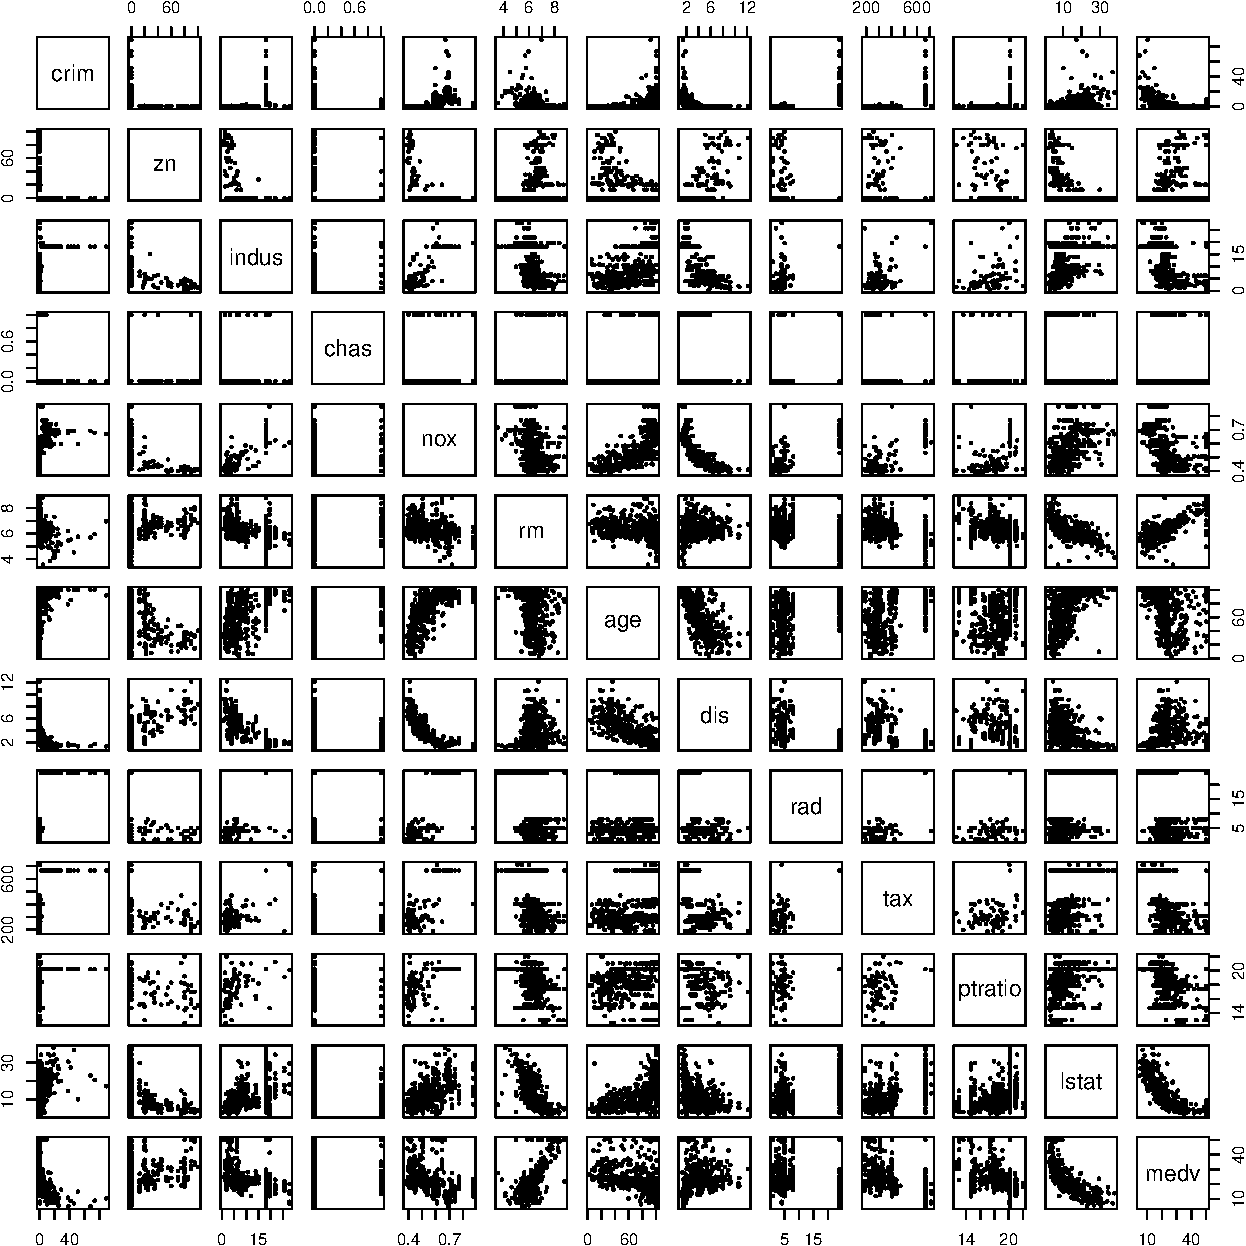
\includegraphics{ch02_exercises_files/figure-latex/pairs-plot-1} \end{center}

A full \(13\times13\) grid is dense, so it helps to know what to look
for rather than eyeball all 78 panels equally. A few patterns stand out
visually and are confirmed by the correlations pulled out in part (c)
below:

\begin{itemize}
\tightlist
\item
  \textbf{\texttt{lstat} vs.~\texttt{medv}}: a clear negative, curved
  (not perfectly linear) relationship --- tracts with a higher share of
  lower-status population have systematically lower home values.
\item
  \textbf{\texttt{rm} vs.~\texttt{medv}}: a positive relationship ---
  more rooms per dwelling tends to mean higher home value, which makes
  intuitive sense (bigger houses cost more).
\item
  \textbf{\texttt{nox} vs.~\texttt{indus}} and \textbf{\texttt{nox}
  vs.~\texttt{age}}: positive relationships --- tracts with more
  industrial land use, and with older housing stock, tend to have higher
  nitrogen oxide pollution.
\item
  \textbf{\texttt{tax} vs.~\texttt{rad}}: a striking pattern where many
  tracts cluster at one very high value of \texttt{rad} (the
  accessibility-to-highways index) paired with a high, fairly constant
  \texttt{tax} rate --- visible as a dense vertical/ horizontal band
  rather than a smooth trend.
\item
  \textbf{\texttt{dis} vs.~\texttt{nox}, \texttt{age}, \texttt{indus}}:
  negative relationships --- tracts farther from Boston's employment
  centers tend to be less industrial, have newer housing, and lower
  pollution (consistent with them being more suburban).
\end{itemize}

\subsection{(c) Predictors associated with per-capita crime
rate}\label{c-predictors-associated-with-per-capita-crime-rate}

\begin{Shaded}
\begin{Highlighting}[]
\FunctionTok{sort}\NormalTok{(}\FunctionTok{cor}\NormalTok{(Boston)[, }\StringTok{"crim"}\NormalTok{])}
\end{Highlighting}
\end{Shaded}

\begin{verbatim}
##        medv         dis          rm          zn        chas     ptratio 
## -0.38830461 -0.37967009 -0.21924670 -0.20046922 -0.05589158  0.28994558 
##         age       indus         nox       lstat         tax         rad 
##  0.35273425  0.40658341  0.42097171  0.45562148  0.58276431  0.62550515 
##        crim 
##  1.00000000
\end{verbatim}

Yes --- several predictors show a meaningful relationship with
\texttt{crim}:

\begin{itemize}
\tightlist
\item
  \textbf{\texttt{rad}} (r \(\approx\) 0.63) and \textbf{\texttt{tax}}
  (r \(\approx\) 0.58) are the strongest --- tracts with better highway
  accessibility and higher property tax rates tend to have notably
  higher crime rates. This is really one pattern more than two, since
  \texttt{rad} and \texttt{tax} are themselves highly correlated
  (visible as that dense cluster in part (b)) --- a small subset of
  tracts with maxed-out \texttt{rad} and \texttt{tax} values are
  dragging crime up with them.
\item
  \textbf{\texttt{lstat}} (r \(\approx\) 0.46) and \textbf{\texttt{nox}}
  (r \(\approx\) 0.42) are moderately positively associated --- tracts
  with more lower-status population and more air pollution tend to have
  higher crime.
\item
  \textbf{\texttt{medv}} (r \(\approx\) -0.39) and \textbf{\texttt{dis}}
  (r \(\approx\) -0.38) are moderately negatively associated --- higher
  home values and greater distance from employment centers both
  correspond to lower crime.
\end{itemize}

Note these are all linear (Pearson) correlations; the true relationships
may well be non-linear, so these numbers indicate \emph{association},
not necessarily the full shape of the relationship.

\subsection{(d) Notably high crime, tax, or pupil-teacher tracts;
ranges}\label{d-notably-high-crime-tax-or-pupil-teacher-tracts-ranges}

\begin{Shaded}
\begin{Highlighting}[]
\FunctionTok{sapply}\NormalTok{(Boston[, }\FunctionTok{c}\NormalTok{(}\StringTok{"crim"}\NormalTok{, }\StringTok{"tax"}\NormalTok{, }\StringTok{"ptratio"}\NormalTok{)], range)}
\end{Highlighting}
\end{Shaded}

\begin{verbatim}
##          crim tax ptratio
## [1,]  0.00632 187    12.6
## [2,] 88.97620 711    22.0
\end{verbatim}

\begin{Shaded}
\begin{Highlighting}[]
\FunctionTok{sapply}\NormalTok{(Boston[, }\FunctionTok{c}\NormalTok{(}\StringTok{"crim"}\NormalTok{, }\StringTok{"tax"}\NormalTok{, }\StringTok{"ptratio"}\NormalTok{)], summary)}
\end{Highlighting}
\end{Shaded}

\begin{verbatim}
##              crim      tax  ptratio
## Min.     0.006320 187.0000 12.60000
## 1st Qu.  0.082045 279.0000 17.40000
## Median   0.256510 330.0000 19.05000
## Mean     3.613524 408.2372 18.45553
## 3rd Qu.  3.677083 666.0000 20.20000
## Max.    88.976200 711.0000 22.00000
\end{verbatim}

\begin{itemize}
\tightlist
\item
  \textbf{\texttt{crim}} ranges from \textbf{0.006 to 88.98} --- an
  enormous spread. The median tract has a crime rate near 0.26, so a
  handful of tracts (crime rate in the 40s--80s) are extreme outliers
  pulling the mean well above the median --- most tracts are low-crime,
  with a small number of very high-crime tracts.
\item
  \textbf{\texttt{tax}} ranges from \textbf{187 to 711} (per \$10,000 of
  property value). There's a visible cluster of tracts sitting right at
  the maximum (666), the same cluster seen in the
  \texttt{tax}--\texttt{rad} pattern from part (b) --- so while the
  \emph{range} is wide, a meaningful subgroup of tracts is bunched at
  the top of it.
\item
  \textbf{\texttt{ptratio}} ranges from \textbf{12.6 to 22.0} --- a
  comparatively narrow spread on an absolute scale, though a
  pupil-teacher ratio of 22 vs.~12.6 is still a substantively large
  difference in school resourcing per student.
\end{itemize}

\subsection{(e) Tracts bounding the Charles
River}\label{e-tracts-bounding-the-charles-river}

\begin{Shaded}
\begin{Highlighting}[]
\FunctionTok{sum}\NormalTok{(Boston}\SpecialCharTok{$}\NormalTok{chas)}
\end{Highlighting}
\end{Shaded}

\begin{verbatim}
## [1] 35
\end{verbatim}

\textbf{35} of the 506 census tracts bound the Charles River
(\texttt{chas\ ==\ 1}).

\subsection{(f) Median pupil-teacher
ratio}\label{f-median-pupil-teacher-ratio}

\begin{Shaded}
\begin{Highlighting}[]
\FunctionTok{median}\NormalTok{(Boston}\SpecialCharTok{$}\NormalTok{ptratio)}
\end{Highlighting}
\end{Shaded}

\begin{verbatim}
## [1] 19.05
\end{verbatim}

The median pupil-teacher ratio across tracts is \textbf{19.05}.

\subsection{(g) Tract with the lowest median home
value}\label{g-tract-with-the-lowest-median-home-value}

\begin{Shaded}
\begin{Highlighting}[]
\FunctionTok{which.min}\NormalTok{(Boston}\SpecialCharTok{$}\NormalTok{medv)}
\end{Highlighting}
\end{Shaded}

\begin{verbatim}
## [1] 399
\end{verbatim}

\begin{Shaded}
\begin{Highlighting}[]
\NormalTok{Boston[}\FunctionTok{which.min}\NormalTok{(Boston}\SpecialCharTok{$}\NormalTok{medv), ]}
\end{Highlighting}
\end{Shaded}

\begin{verbatim}
##        crim zn indus chas   nox    rm age    dis rad tax ptratio lstat medv
## 399 38.3518  0  18.1    0 0.693 5.453 100 1.4896  24 666    20.2 30.59    5
\end{verbatim}

Tract \textbf{399} has the lowest \texttt{medv} at \textbf{\$5,000} ---
far below the data set's minimum-to-typical range (the next
visualization makes the point concretely: this tract sits at the very
bottom of the \texttt{medv} distribution while most other predictors sit
near the \emph{top} of their own ranges).

\begin{Shaded}
\begin{Highlighting}[]
\NormalTok{idx }\OtherTok{\textless{}{-}} \FunctionTok{which.min}\NormalTok{(Boston}\SpecialCharTok{$}\NormalTok{medv)}
\FunctionTok{sapply}\NormalTok{(}\FunctionTok{names}\NormalTok{(Boston), }\ControlFlowTok{function}\NormalTok{(v) }\FunctionTok{round}\NormalTok{(}\DecValTok{100} \SpecialCharTok{*} \FunctionTok{mean}\NormalTok{(Boston[[v]] }\SpecialCharTok{\textless{}=}\NormalTok{ Boston[idx, v]), }\DecValTok{1}\NormalTok{))}
\end{Highlighting}
\end{Shaded}

\begin{verbatim}
##    crim      zn   indus    chas     nox      rm     age     dis     rad     tax 
##    98.8    73.5    88.7    93.1    85.8     7.7   100.0     5.7   100.0    99.0 
## ptratio   lstat    medv 
##    88.9    97.8     0.4
\end{verbatim}

Interpreting these as percentile ranks within the full data set, tract
399 is a striking outlier profile: it sits at the \textbf{100th
percentile for \texttt{age}} (essentially all owner-occupied units built
before 1940) and \textbf{\texttt{rad}} (maximum highway accessibility),
the \textbf{99th percentile for \texttt{tax}}, the \textbf{98.8th
percentile for \texttt{crim}}, and the \textbf{97.8th percentile for
\texttt{lstat}} --- while its \texttt{rm} (rooms per dwelling) is only
at the 7.7th percentile and its \texttt{dis} (distance to employment
centers) at the 5.7th percentile. In short: old housing stock, very high
crime and tax burden, small homes, low-status population, and close to
the urban core --- a textbook combination for depressed home values, and
consistent with the associations found in part (c).

\subsection{(h) Tracts averaging more than seven / eight
rooms}\label{h-tracts-averaging-more-than-seven-eight-rooms}

\begin{Shaded}
\begin{Highlighting}[]
\FunctionTok{sum}\NormalTok{(Boston}\SpecialCharTok{$}\NormalTok{rm }\SpecialCharTok{\textgreater{}} \DecValTok{7}\NormalTok{)}
\end{Highlighting}
\end{Shaded}

\begin{verbatim}
## [1] 64
\end{verbatim}

\begin{Shaded}
\begin{Highlighting}[]
\FunctionTok{sum}\NormalTok{(Boston}\SpecialCharTok{$}\NormalTok{rm }\SpecialCharTok{\textgreater{}} \DecValTok{8}\NormalTok{)}
\end{Highlighting}
\end{Shaded}

\begin{verbatim}
## [1] 13
\end{verbatim}

\begin{Shaded}
\begin{Highlighting}[]
\FunctionTok{summary}\NormalTok{(Boston[Boston}\SpecialCharTok{$}\NormalTok{rm }\SpecialCharTok{\textgreater{}} \DecValTok{8}\NormalTok{, ])}
\end{Highlighting}
\end{Shaded}

\begin{verbatim}
##       crim               zn            indus             chas       
##  Min.   :0.02009   Min.   : 0.00   Min.   : 2.680   Min.   :0.0000  
##  1st Qu.:0.33147   1st Qu.: 0.00   1st Qu.: 3.970   1st Qu.:0.0000  
##  Median :0.52014   Median : 0.00   Median : 6.200   Median :0.0000  
##  Mean   :0.71880   Mean   :13.62   Mean   : 7.078   Mean   :0.1538  
##  3rd Qu.:0.57834   3rd Qu.:20.00   3rd Qu.: 6.200   3rd Qu.:0.0000  
##  Max.   :3.47428   Max.   :95.00   Max.   :19.580   Max.   :1.0000  
##       nox               rm             age             dis       
##  Min.   :0.4161   Min.   :8.034   Min.   : 8.40   Min.   :1.801  
##  1st Qu.:0.5040   1st Qu.:8.247   1st Qu.:70.40   1st Qu.:2.288  
##  Median :0.5070   Median :8.297   Median :78.30   Median :2.894  
##  Mean   :0.5392   Mean   :8.349   Mean   :71.54   Mean   :3.430  
##  3rd Qu.:0.6050   3rd Qu.:8.398   3rd Qu.:86.50   3rd Qu.:3.652  
##  Max.   :0.7180   Max.   :8.780   Max.   :93.90   Max.   :8.907  
##       rad              tax           ptratio          lstat           medv     
##  Min.   : 2.000   Min.   :224.0   Min.   :13.00   Min.   :2.47   Min.   :21.9  
##  1st Qu.: 5.000   1st Qu.:264.0   1st Qu.:14.70   1st Qu.:3.32   1st Qu.:41.7  
##  Median : 7.000   Median :307.0   Median :17.40   Median :4.14   Median :48.3  
##  Mean   : 7.462   Mean   :325.1   Mean   :16.36   Mean   :4.31   Mean   :44.2  
##  3rd Qu.: 8.000   3rd Qu.:307.0   3rd Qu.:17.40   3rd Qu.:5.12   3rd Qu.:50.0  
##  Max.   :24.000   Max.   :666.0   Max.   :20.20   Max.   :7.44   Max.   :50.0
\end{verbatim}

\textbf{64} tracts average more than seven rooms per dwelling, and
\textbf{13} average more than eight.

The 13 tracts with \texttt{rm\ \textgreater{}\ 8} are a notably
\emph{advantaged} subset compared to the data set as a whole: their
median \texttt{crim} (\(\approx\) 0.52) and \texttt{lstat} (\(\approx\)
4.14) are both far below the full data set's medians, and their median
\texttt{medv} (\$48,300) sits near the top of the overall home-value
range (recall the overall \texttt{medv} maximum is \$50,000, likely
censored at that value). In other words, large-home tracts tend to
combine low crime, low lower-status population share, and high home
values --- consistent with the negative \texttt{lstat}--\texttt{medv}
and positive \texttt{rm}--\texttt{medv} relationships seen in part (b).

\end{document}
